
\chapter{Introduction}

%In large companies, it is possible to have dozens or even hundreds of software projects underway at any given point in time. This kind of scale produces new challenges, as well as new opportunities for these companies. Both challenges and opportunities result from the need of the company to successfully understand and exploit their ownership of a portfolio of software projects. 

%Single project management is easy to achieve from various way. Many software metrics, such as coverage, complexity and file size, provide significant information about a software project. But it is reported that, almost all metrics have deficiency when judge a state of a project with only one or two of them. Therefore, people usually trend to look into more metrics to understand a project. However, while the number of projects increases as well as the number of metrics increases, the data to read inflates rapidly and become overwhelming.

%In order to address this issue and achieve efficient governance over large number of projects, we introduce an analysis tool called Software Intensive Care Unit. It is from the idea of intensive care unit in hospitals where patients are placed with sensors from sophisticated machines and they are consistently monitoring the patients' various vital sign such as pulse, breathe, etc. Similarly, Software Intensive Care Unit(SICU) provides various software metrics, each of which reveals one aspect of the project. These metrics are the vital signs of a software project. With all these vital signs together, users can have a fast but complete view of the projects, leading to easier understanding of projects and make better decisions and practice. Though one might argue that software projects' performance cannot be simply judged by a set of metrics, the case is the same in medicine. A doctor will not simply diagnose a patient by those vital signs, but it is undoubtedly that the medical intensive care unit helps the diagnosis a lot, so it is the software intensive care unit.

%However, to build up the SICU is a great challenge. Both what data to show and how to show them are essential to successfully set up a SICU that offer enough insight into the most interesting aspect of the projects without too much data overwhelming. Moreover, interesting things are various from different situation. Some setting may be common over projects and organization, but we don't believe there is a golden rule for all projects. So system should give users the capability to customize as their need.


\section{The Problem}
Software metrics are one of the essential tool for performance measuring and quality control. But they are not comprehensive enough to make judgement with only one or two. So, we need to utilize multiple metrics in order to acquire insight of the health state of the software project. The more software metrics, the more comprehensive insight, but also the more effort it will need to collect measure data and interpret values. My research tries to overcome this challenge by developing a system to help observer the health state of the software project from multiple software metrics in an effective way.

\section{Software Intensive Care Unit Approach}
What is SICU

\section{Thesis Claim}
We claim it is the most powerful tool ever in the world! =P

\section{Evaluation}
We evaluate in a classroom.

\section{Thesis Structure}
Here is a paragraph that saying the same thing as TOC.

\chapter{Related Work}
This chapter presents some related work of my research.

First part discusses previous research on empirical software engineering concepts. Most previous researches on measurement-based software engineering focus on methodology. Effective approaches are developed and deployed in actual practice. However, the lack of automation adds significant overhead to developers, thus lead the impression that they are hard. Research of Hackystat and Software ICU is towards the 3rd generation of approaches to PSP metrics that automate data collection and analyze\cite{csdl2-02-07}.

Second part discusses three recent research that focus on automated data collection. Two of them mainly focus on introduction level programming course and not very suitable to senior software development or professional settings. The third one is very similar to Hackystat and has related industry studies.

%Third part discusses some commercial ``dashboards'' for software project data. Software ICU is one example of a project dashboard. However, it differs from commercial approaches with its intensive metrics, high extensibility and open source development and distribution. 

Last part discusses two previous related case studies of Hackystat system to provide some insight into the development history of Hackystat.

\section {TSP/PSP}
The Personal Software Process(PSP)\cite{book:psp} and the Team Software Process(TSP)\cite{book:tsp} are among the most extensively studied approaches for measurement-based software engineering. They were developed by Watts Humphrey to teach students (in university and industry alike) to the use of large scale methods based on the Capability Maturity Model (CMM). It scales down industrial software practices to fit the needs of small scale program development. Software processes and software engineering disciplines are gradually introduced through small program projects (e.g. course assignment projects). The PSP maturity progression is shown in \autoref{fig:PSP-Evo}. Students gather both process and product measures of each involved projects. By comparing the measurement result to their original planning, they understand their programming habits, both pros and cons, and refine their process to higher level of maturity level.

\begin{figure}[htbp] %  figure placement: here, top, bottom, or page
   \centering
   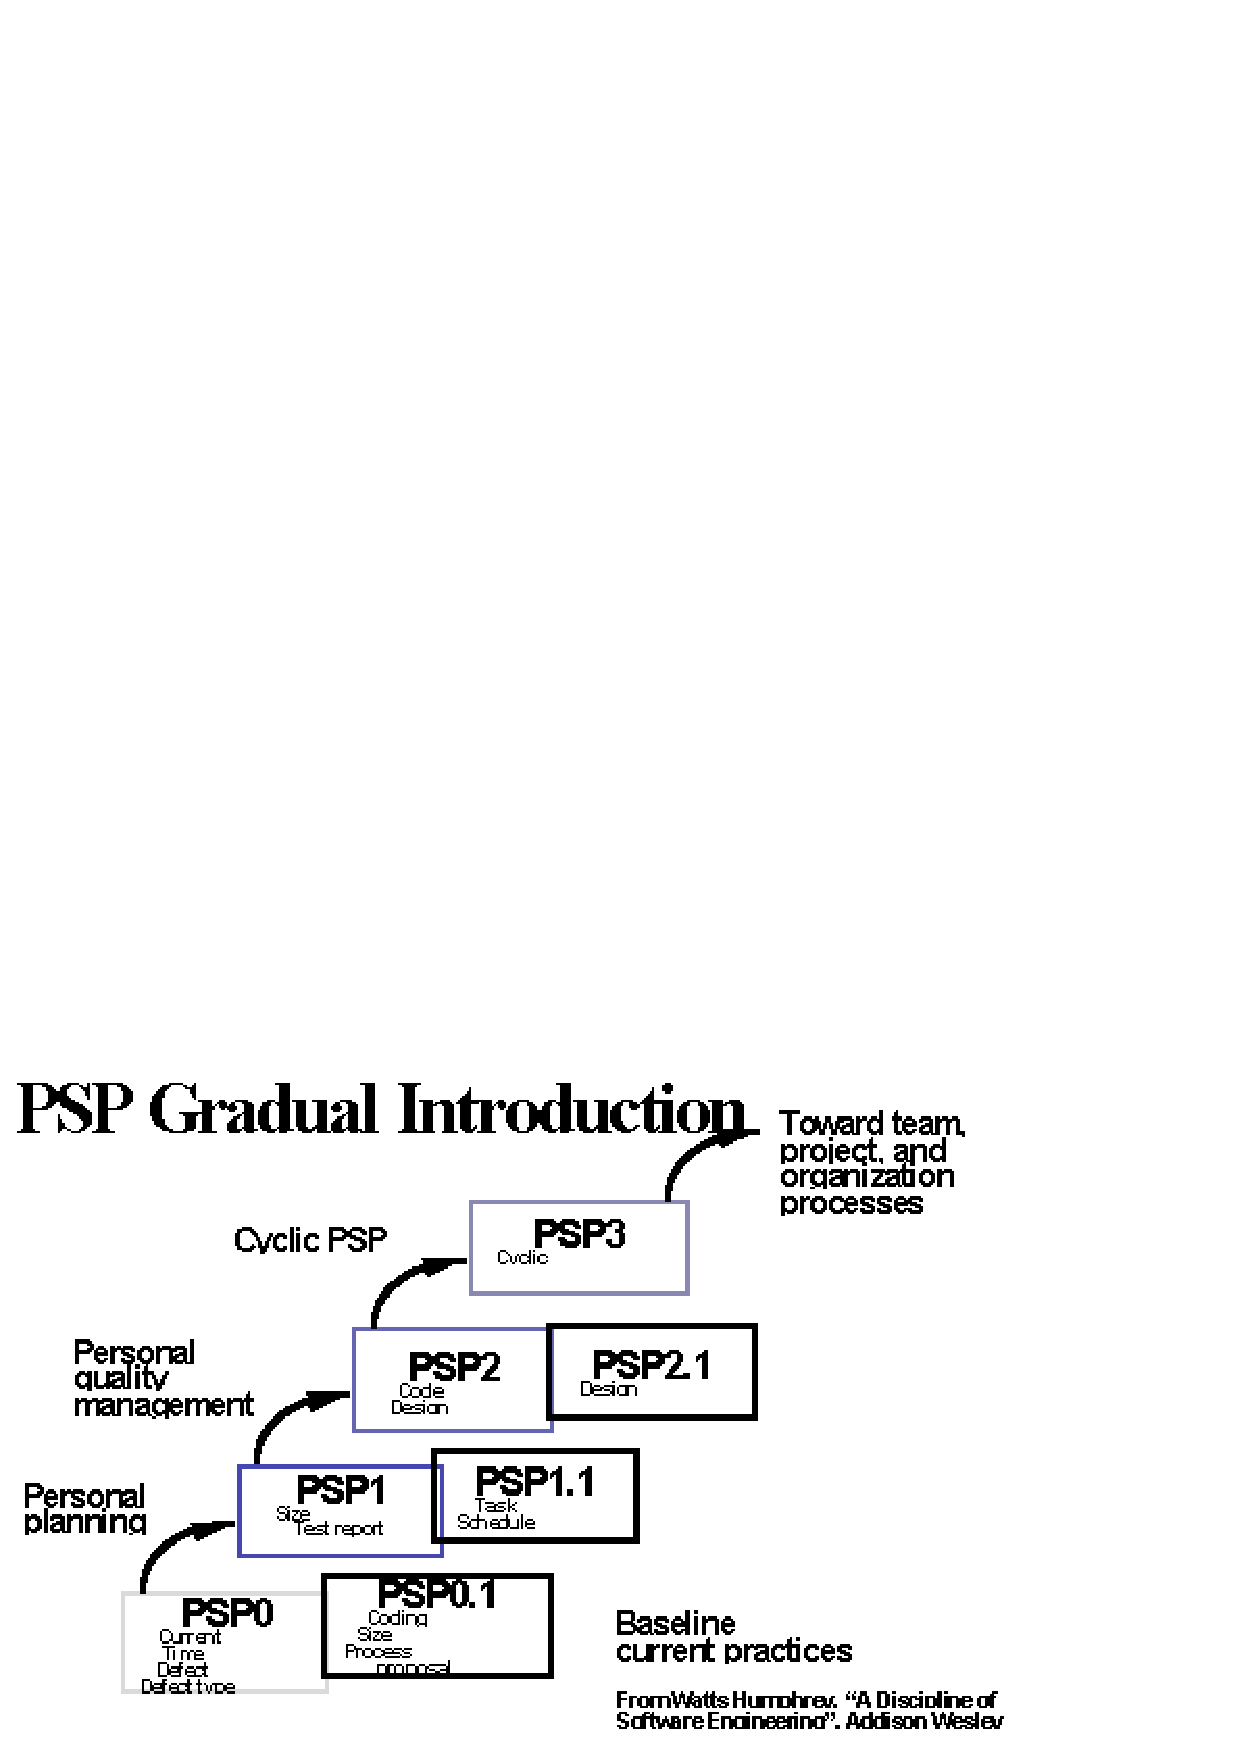
\includegraphics[height=20em]{PSP-Evo} 
   \caption{Progression of PSP}
   \label{fig:PSP-Evo}
\end{figure}

PSP/TSP is effective in both academic education as well as industrial application. (more about related research)

Major drawback is lack of automation. Developers have to manually record their process and product data (mostly the development time and number of defects). The high overhead of data collection raises a barrier to its introduction and adoption. Additionally, it is not easy to ``digest'' the data. Developers have to manually analyze their logged data in order to understand the their performance, then be able to improve it.

On the contrary, Software ICU provide a higher level of automation in tracking and analyzing software process and product data.


\section {Research Based on Automated Data Collection}
Project ClockIt and Retina are two recent researches based on automated data collection to support entry-level programming courses, while PROM is the most similar research to Hackystat.

\subsection {Project ClockIt and Retina}
Project ClockIt provides a data logger as BlueJ\footnote{``BlueJ is an integrated Java environment specifically designed for introductory teaching.'' --Quoted from \url{http://www.bluej.org/about/what.html}}
 extension. It logs developer's open/close of project and package, file change and delete and compilation results. Data is logged to local file and later send to a database via internet. A data visualizer integrated into BlueJ is available to view data about the current project. \autoref{fig:clockit} shows an example of this visualizer. Data stored in database is used for statistic analysis such as class averages. A web interface is also available to instructors to view the individual data of their students and class average analysis data.

\begin{figure}[htbp] %  figure placement: here, top, bottom, or page
   \centering
   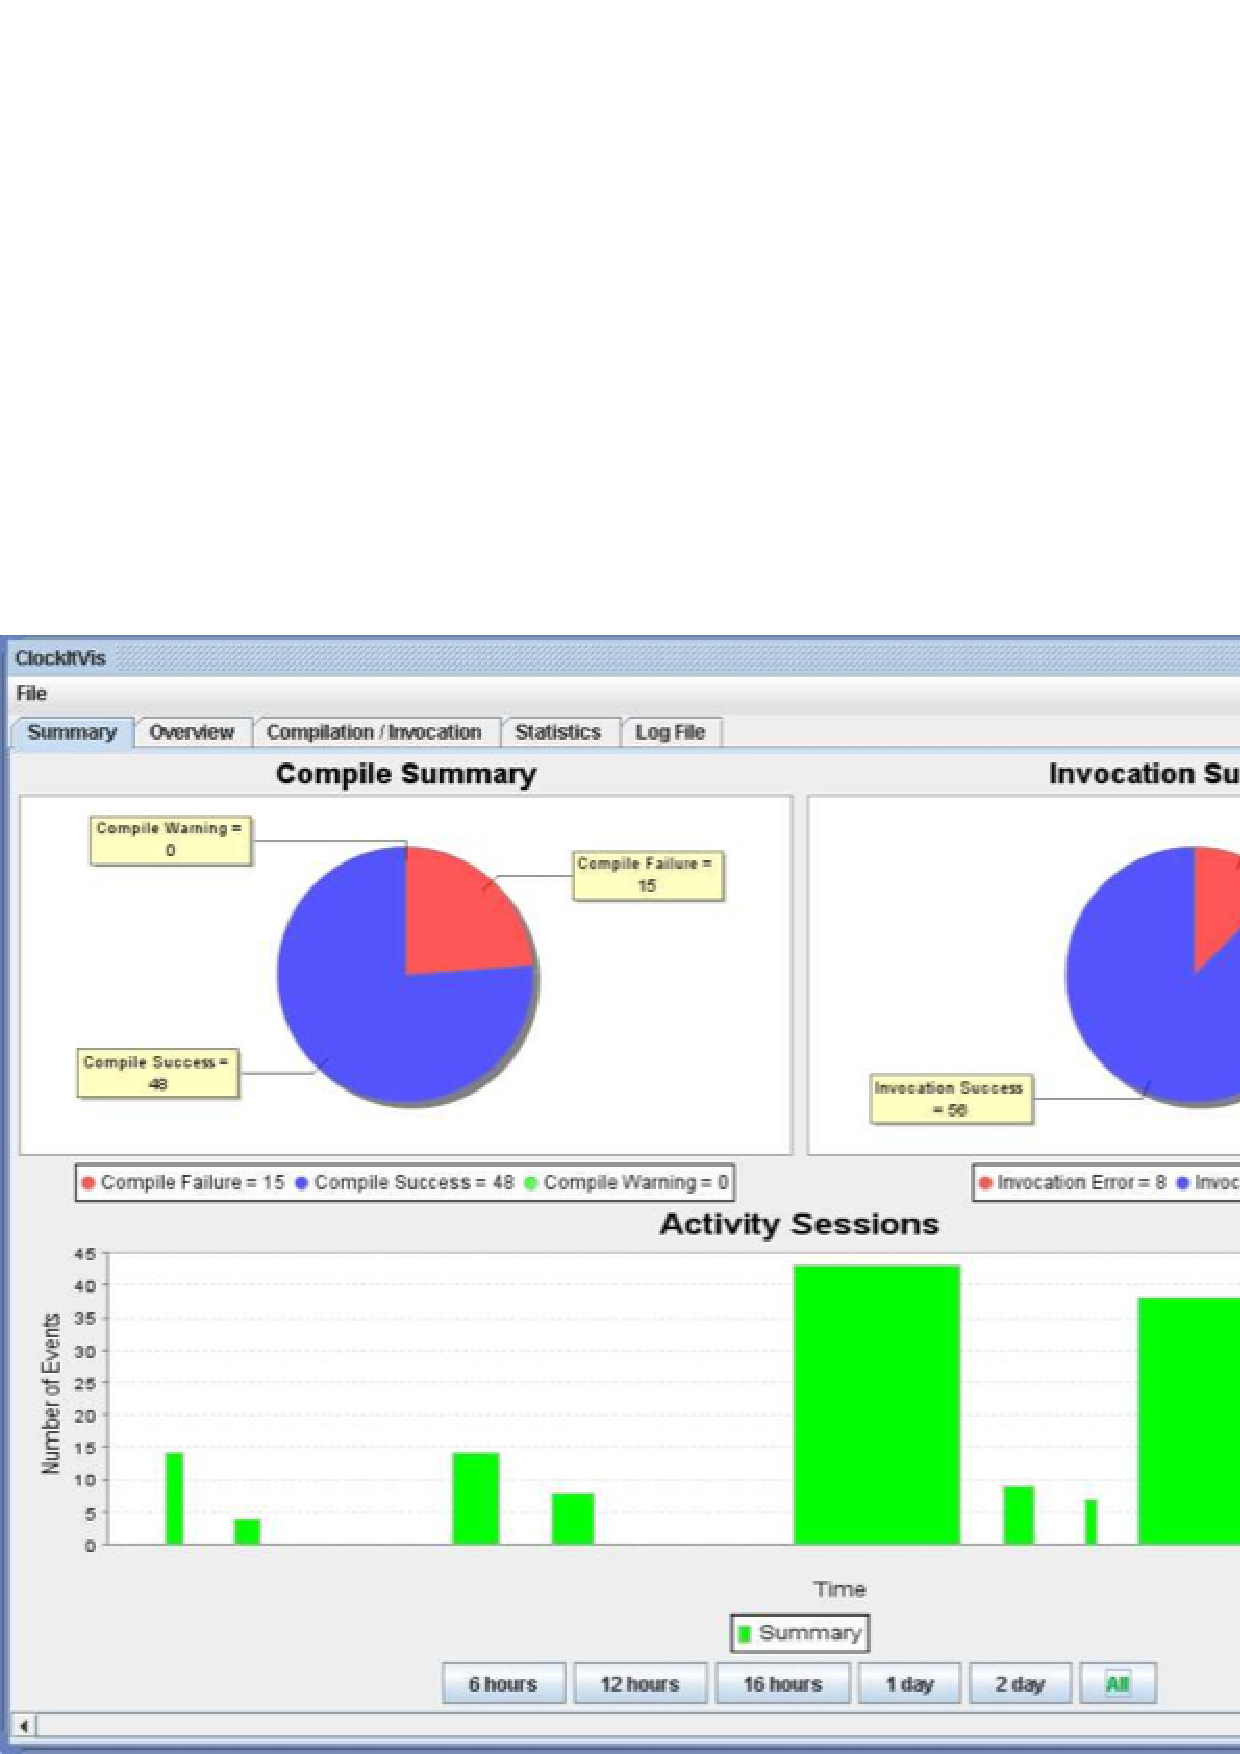
\includegraphics[height=20em]{clockit} 
   \caption{ClockIt BlueJ Data Visualizer summary}
   \label{fig:clockit}
\end{figure}

Closely related to ClockIt, Retina also provides automated data collection. Though Retina provide more tool support (BlueJ, Eclipse and command-line compiler), it focuses on a even smaller area of programming events: the compilation. It gather data from students' compilation events, mostly compilation errors. In additional to its data viewer (see \autoref{fig:retina}), it also provides a recommendation tool for students. The tool use instant messaging (IM) to give students approximated recommendation of amount of time for the upcoming assignment, and the compilation errors one is likely to make. These are based on both the student's previous data and the data from courses of previous semesters. 

\begin{figure}[htbp]
     \centering
     \subfigure[Retina Instructor Viewer]{
          \label{fig:retina-teacher}
          \includegraphics[width=.48\textwidth]{retina-teacher}}
     \subfigure[Retina Student Viewer]{
          \label{fig:retina-teacher}
          \includegraphics[width=.48\textwidth]{retina-student}}
          
     \caption{Data viewers of Retina.}
     \label{fig:retina}
\end{figure}

The difference between these two research and Software ICU is that they are focus only on introductory level courses, where compilation is the interesting development event. In other hand, their relatively easier configuration complements one of the major short-coming of Hackystat and Software ICU, which is also one of the direction we are going to improve. While neither of them provide good extensibility, they are unlikely to be useful in advanced programming situations like advanced programming course or professional setting.

\subsection {PROM}
PRO Metric (PROM) \cite{prom03} is the system that most similar to Hackystat. PROM is a software system for collecting process and product metrics in a software company. It is initiated and driven by the demand of the company, and thus the research is focus on industry setting. It is designed to work fully automatically without any interaction with the user in order to get reliable and accurate data about company internal workflows and development processes. It is organized in a sequence of interconnected components, communicate using SOAP protocol. Similar to sensors in Hackystat, it has plugins for many different applications, including IDEs, word processing tools, email clients, and issue tracking systems, to collect data. Data then is transit to plugin server to extract metric, then the results are sent to PROM server to store into database. \autoref{fig:promarchitecture} shows the overview of PROM's architecture.

\begin{figure}[htbp]
     \centering
     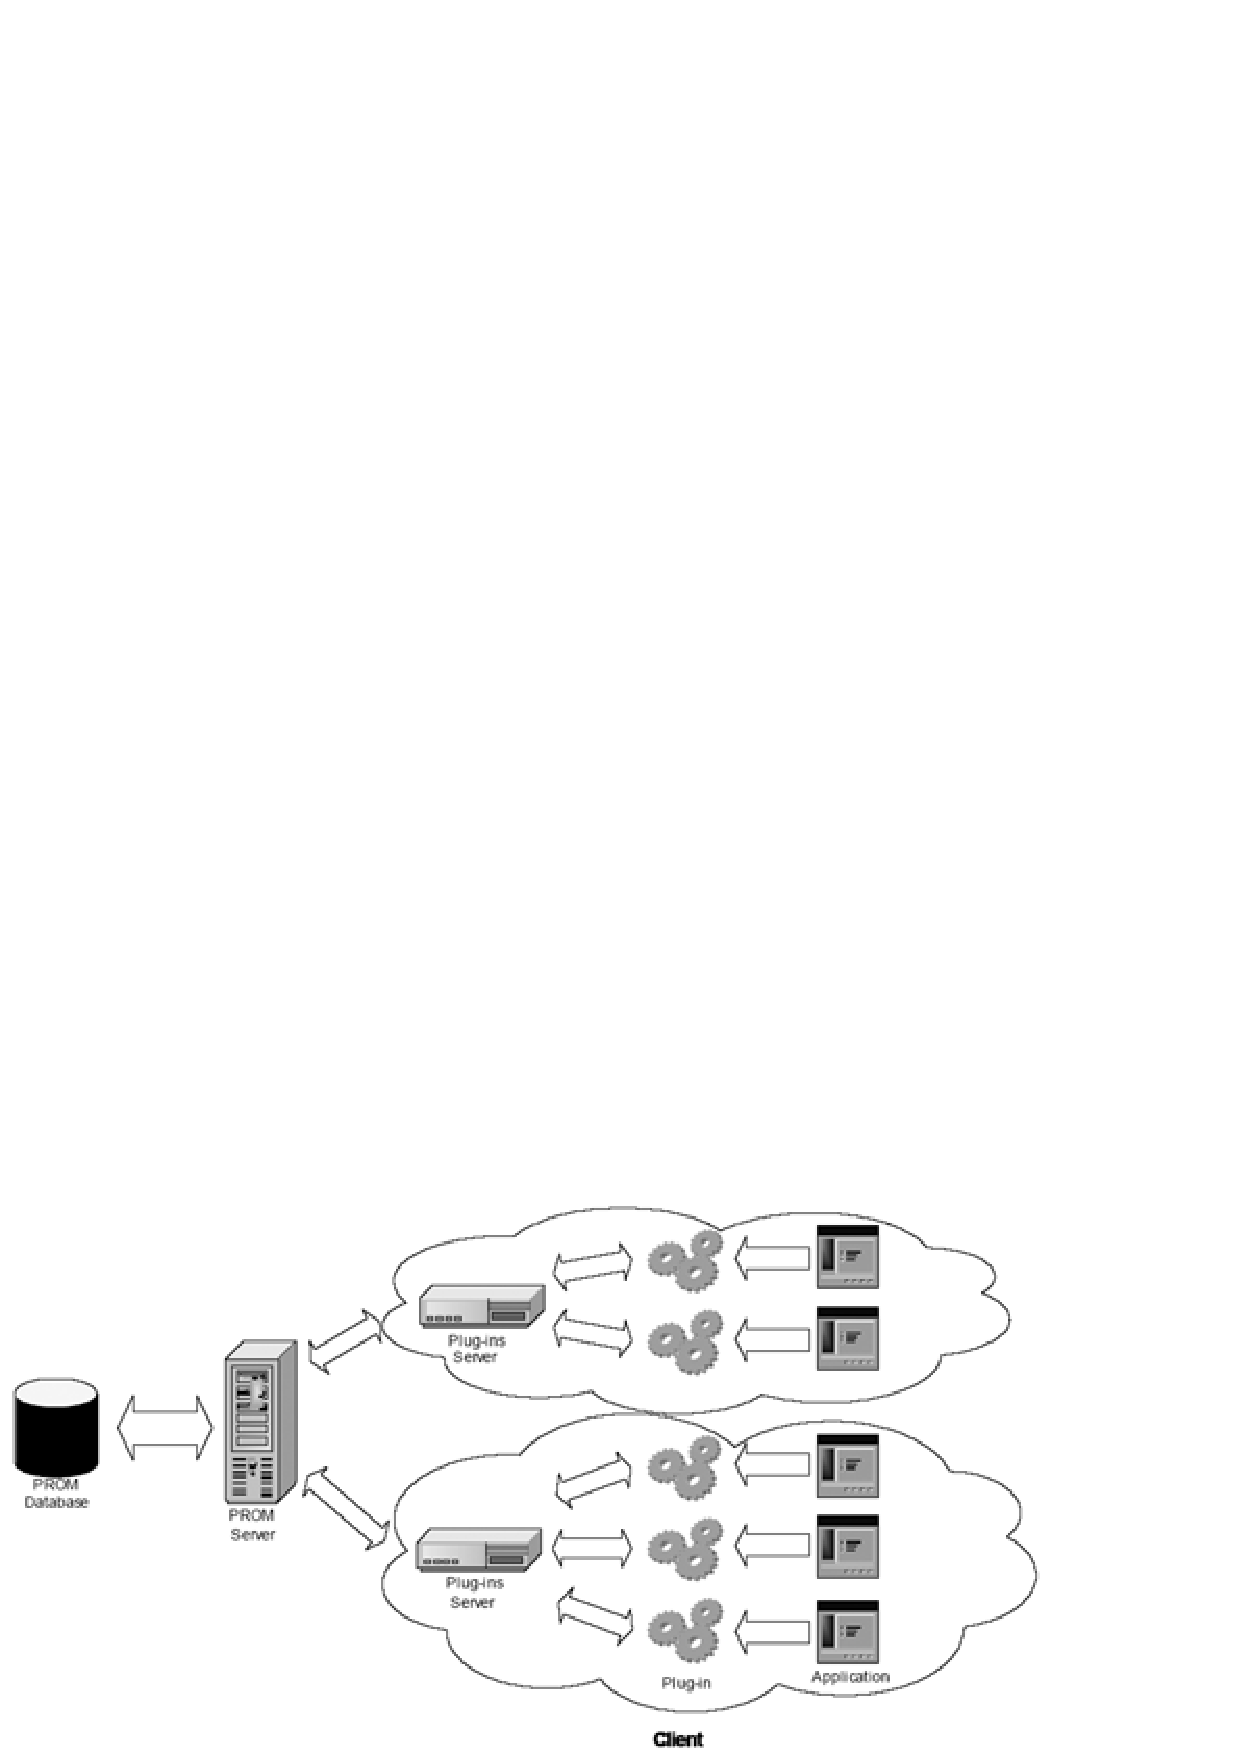
\includegraphics[width=.48\textwidth]{promarchitecture}
     \caption{Architecture of the PROM system}
     \label{fig:promarchitecture}
\end{figure}

PROM categorize users into 3 roles, developer, team leader, and manager of the team. Each of these role is provided different views of data. Developers have access to their individual, detailed data, the leader to the aggregated data of the whole team, and the manager to project level aggregated data.

Compared to Hackystat, PROM's data is stored as analyzed metrics result while Hackystat stores the raw sensor data, and different data viewers are provided to different groups of users while Hackystat give all users access to all viewers.

Recently, a case study of PROM in industrial environment was published\cite{prom09}. In the study, they discuss the lessons learnt from two year experience of using the PROM system in the IT department of a large company in Italy. Evidence indicates that adopting an AISEMA system requires a long time set-up phrase and need the company and develop team's patience and commitment to succeed, but it will eventually deliver value to the company. 

One of the lessons suggest that data presentation is as important as data accuracy and simplicity, brevity and clarity is preferable. Another lesson suggest that fast aggregated view of data is desired, and users of different roles favor different aggregations, e.g. developers like reports of their daily activities, while team leader and manager like summary views of data on team and project level. Software ICU's simple and fast data presentation and high configurability and extensibility is suitable to address these requirements.

%\section {Software Project Dashboards}
%In software industry, there exists many commercial software project manage dashboards, such as LightHouse, ProjectManager.com dashboard, PivotLink Dashboards, Autotask Project Management and so forth. However, many of them are complete solution of software development business management, including not only software project states management, but also related resource allocation and budget control, etc. As being commercial products, they are not open source. Most importantly, there is few research published about these commercial project dashboards. ``Features'' are advertised as other commercial products, while short-comings are ignored. Thus negative results of their use are unknown. This research of Software ICU contains not only its benefits, but also its negative impact.


\section {Previous Case Studies of Hackystat}
The classroom study presented in this thesis is the third case study of Hackystat system in a classroom setting. 

The first case study is performed in 2003 using an early version of Hackystat\cite{csdl2-03-13}. During that time, Hackystat was only collecting 4 types of metrics (Active Time, Size, Unit Tests and Coverage). The system was oriented around a set of ``Course'' analyses that were tailored to an educational setting. Those analyses summaries of the individual team project metric data to-date in tabular form, and also presented comparisons of all of the course projects\autoref{fig:hackystat2003}. The evaluation shows that the installation of Ant sensors is the most significant barrier to the system. It was too difficult to install if without direct help from the development team. But the overhead of use is relatively low and analyses were usable and useful, while data privacy was uncomfortable for some students.

\begin{figure}[htbp]
   \centering
   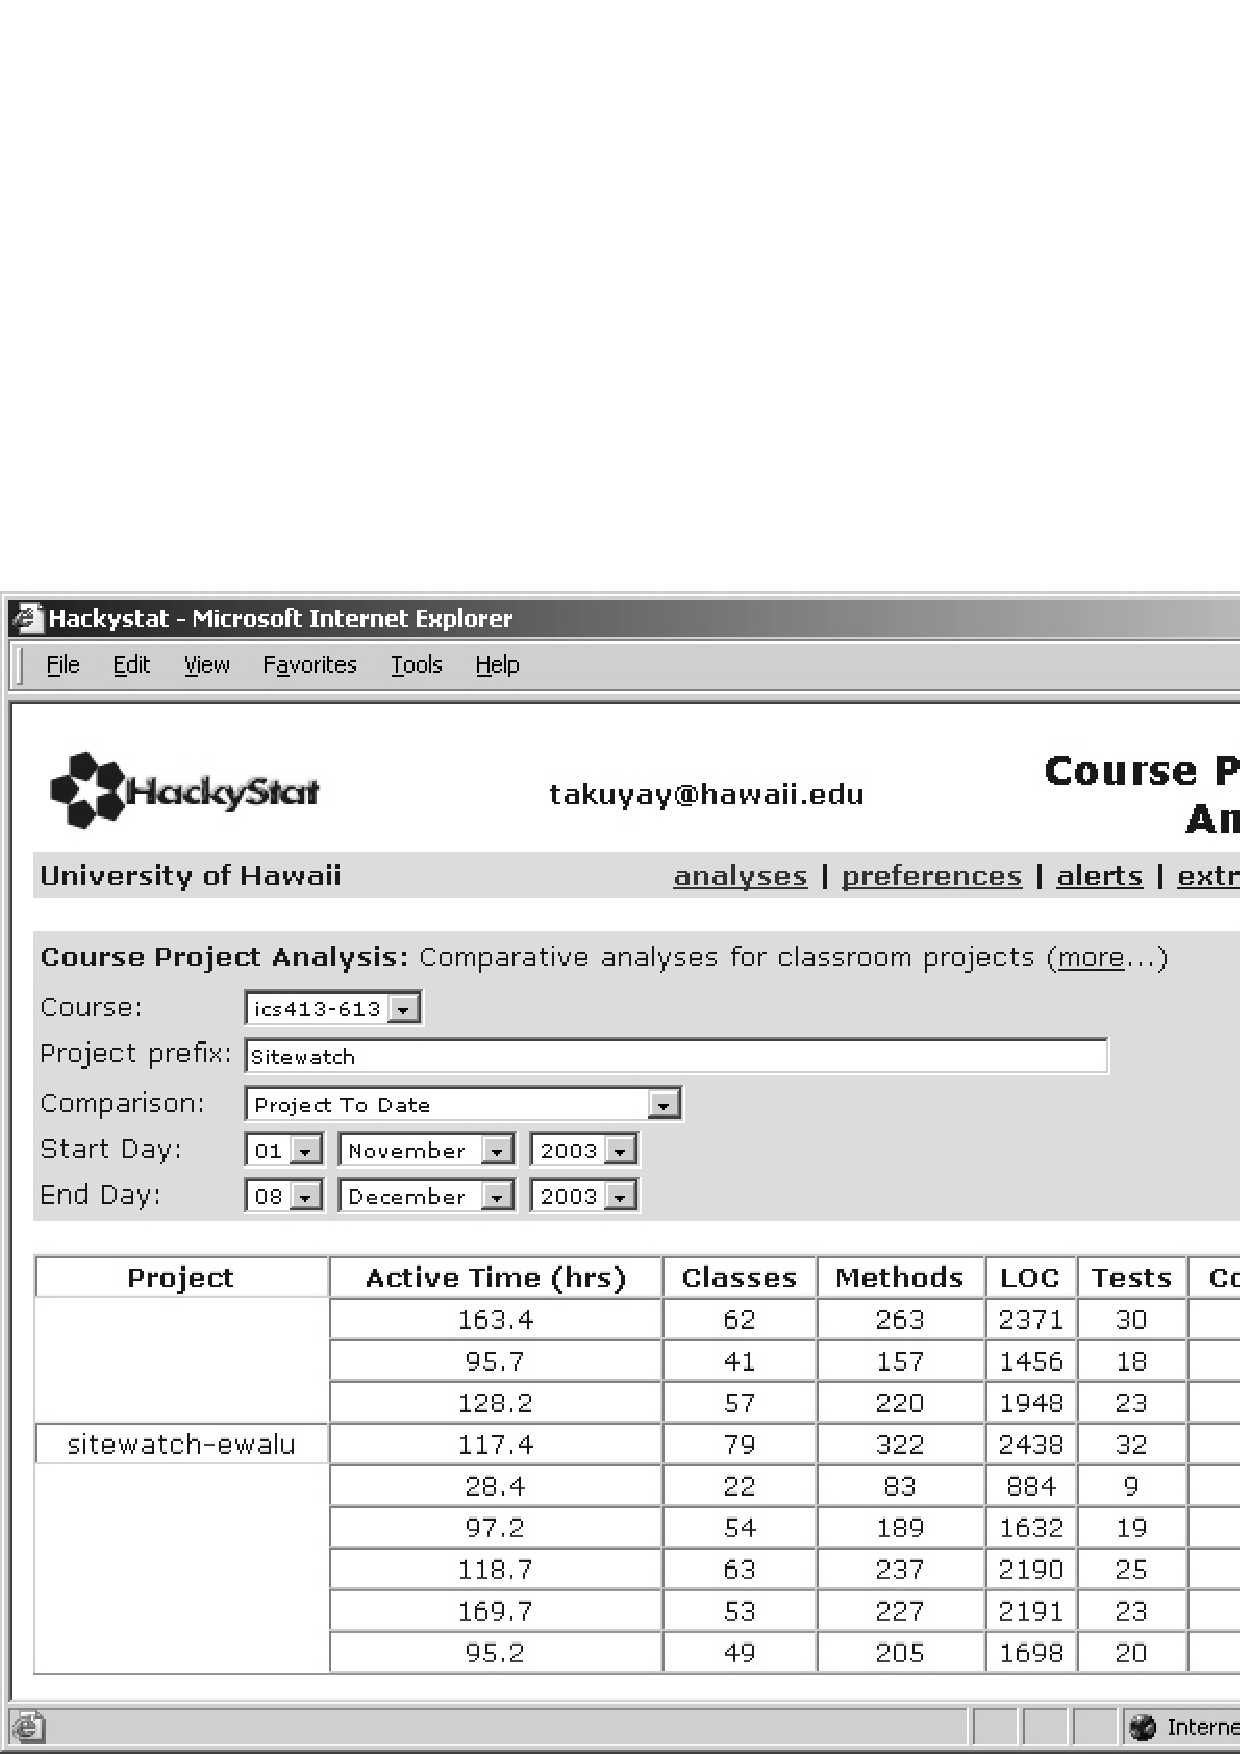
\includegraphics[height=20em]{hackystat2003} 
   \caption{Screenshot of course project to date analysis of Hackystat in 2003}
   \label{fig:hackystat2003}
\end{figure}

The second case study happened in 2006 as a partial replication of the first case study\cite{csdl2-07-02}. The Hackystat had undergone significant change from 2003 to 2006. The sensor installation, which is the major barrier to the system in 2003, was automated by the hackyInstaller GUI, which greatly lower the overhand of configuration for developers. The evaluation also shows significant drop in sensor installation difficulty. However, the new sophisticated Telemetry analysis \autoref{fig:hackystat2006} and its complex user interface raise the difficulty of using it and interpreting data, lead to slightly drop of usability and professional feasibility.

\begin{figure}[htbp]
   \centering
   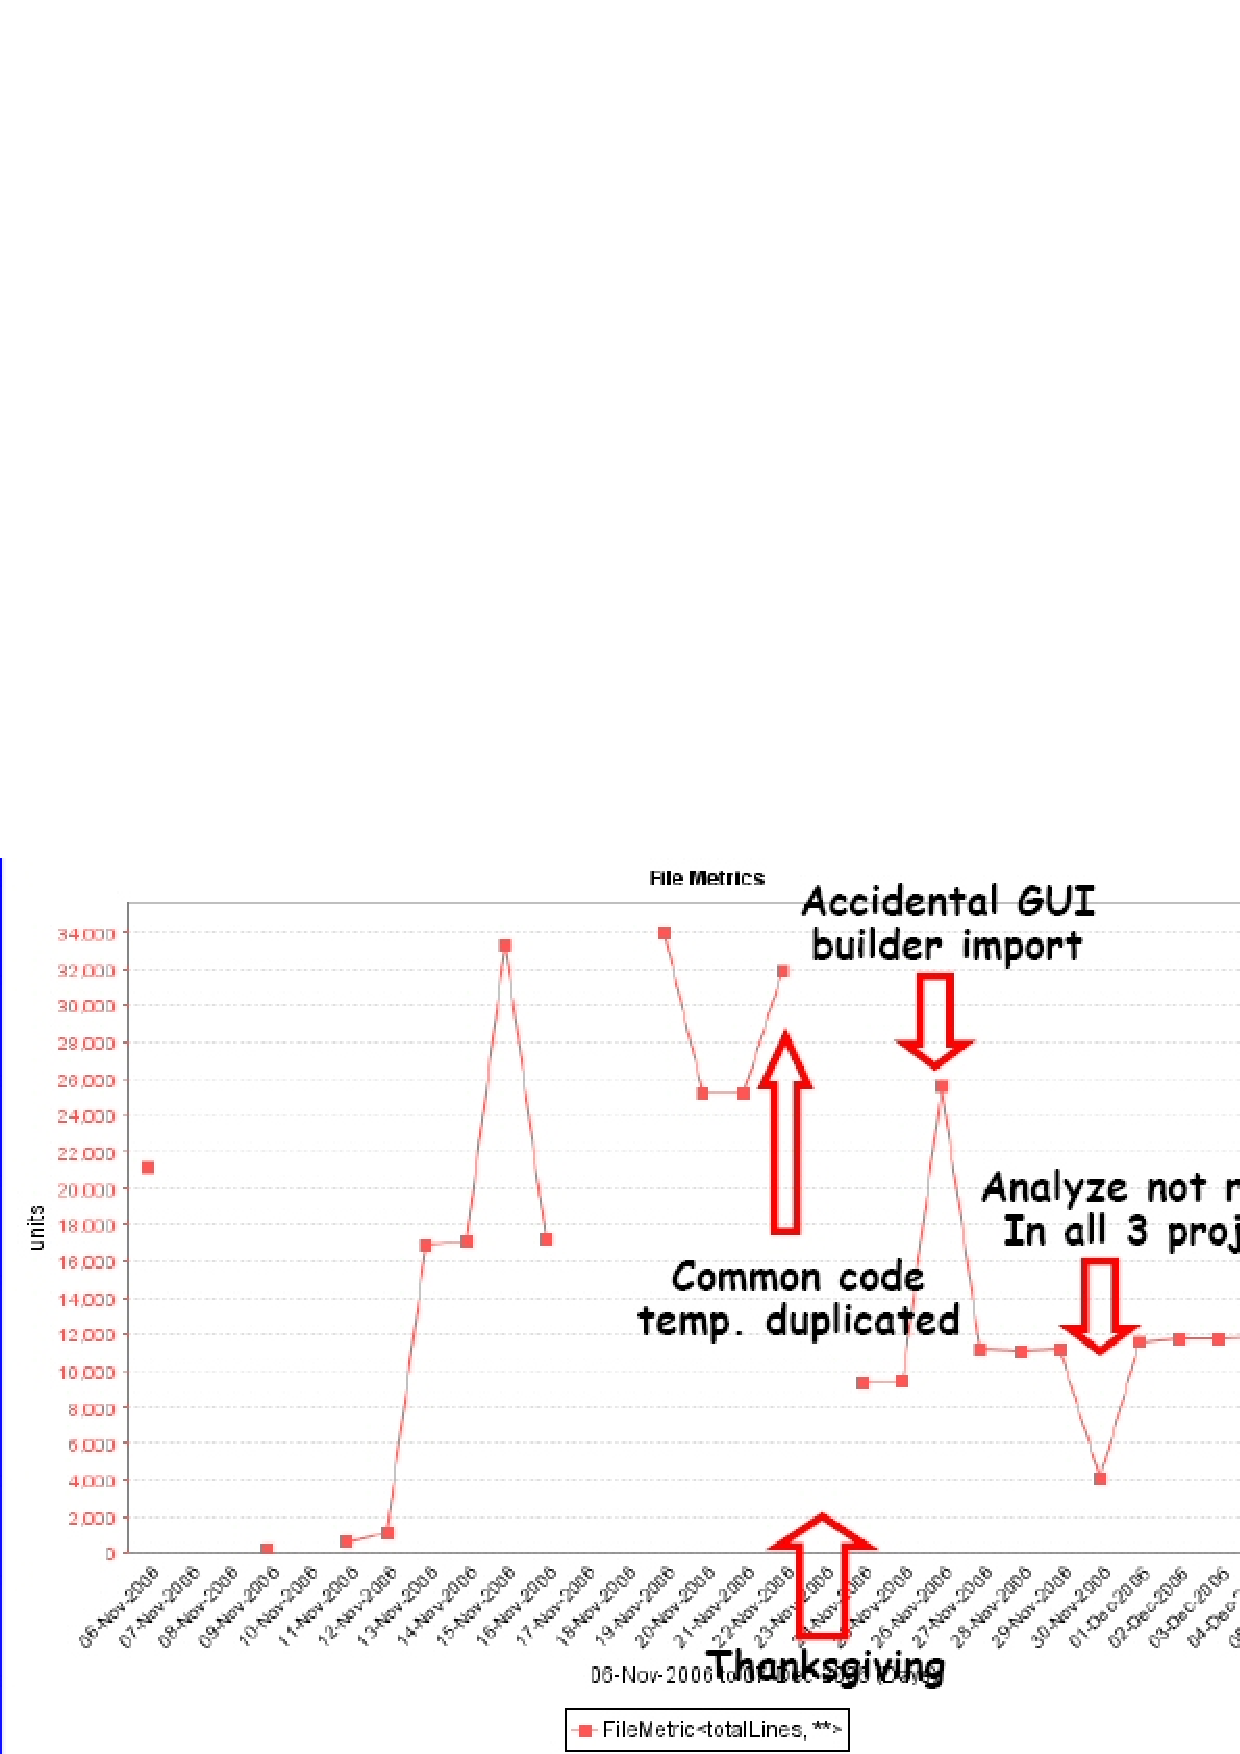
\includegraphics[height=20em]{hackystat2006} 
   \caption{Screenshot of file-metric telemetry analysis of Hackystat in 2006}
   \label{fig:hackystat2006}
\end{figure}

In 2007, Hackystat has been re-implemented to a new architecture version. Adopting the service-oriented architecture enable us to design multiple user interface separately from the kernel components. The Software ICU is built upon a new web-based UI called Project Browser, and the classroom study is also based on this user interface.


\chapter{Hackystat}
In this research, I utilize Hackystat to implement the Software ICU. This chapter briefly introduce the Hackystat system, which was invented by Professor Philip M. Johnson, in the Collaborative Software Development Laboratory, Department of Information and Computer Sciences, University of Hawaii at Manoa. 
 
\section{Hackystat Framework}
Hackystat is an open source framework for collection, analysis, visualization, interpretation, annotation, and dissemination of software development process and product data. Hackystat consist of many software services that communicate using REST architectural principles\cite{wiki:restful}. These software services can be categorize into 4 groups, sensors, data repository, analysis services and viewers. \autoref{fig:hackystat-architecture} shows the architecture of Hackystat system. 

\begin{figure}[htbp]
   \centering
   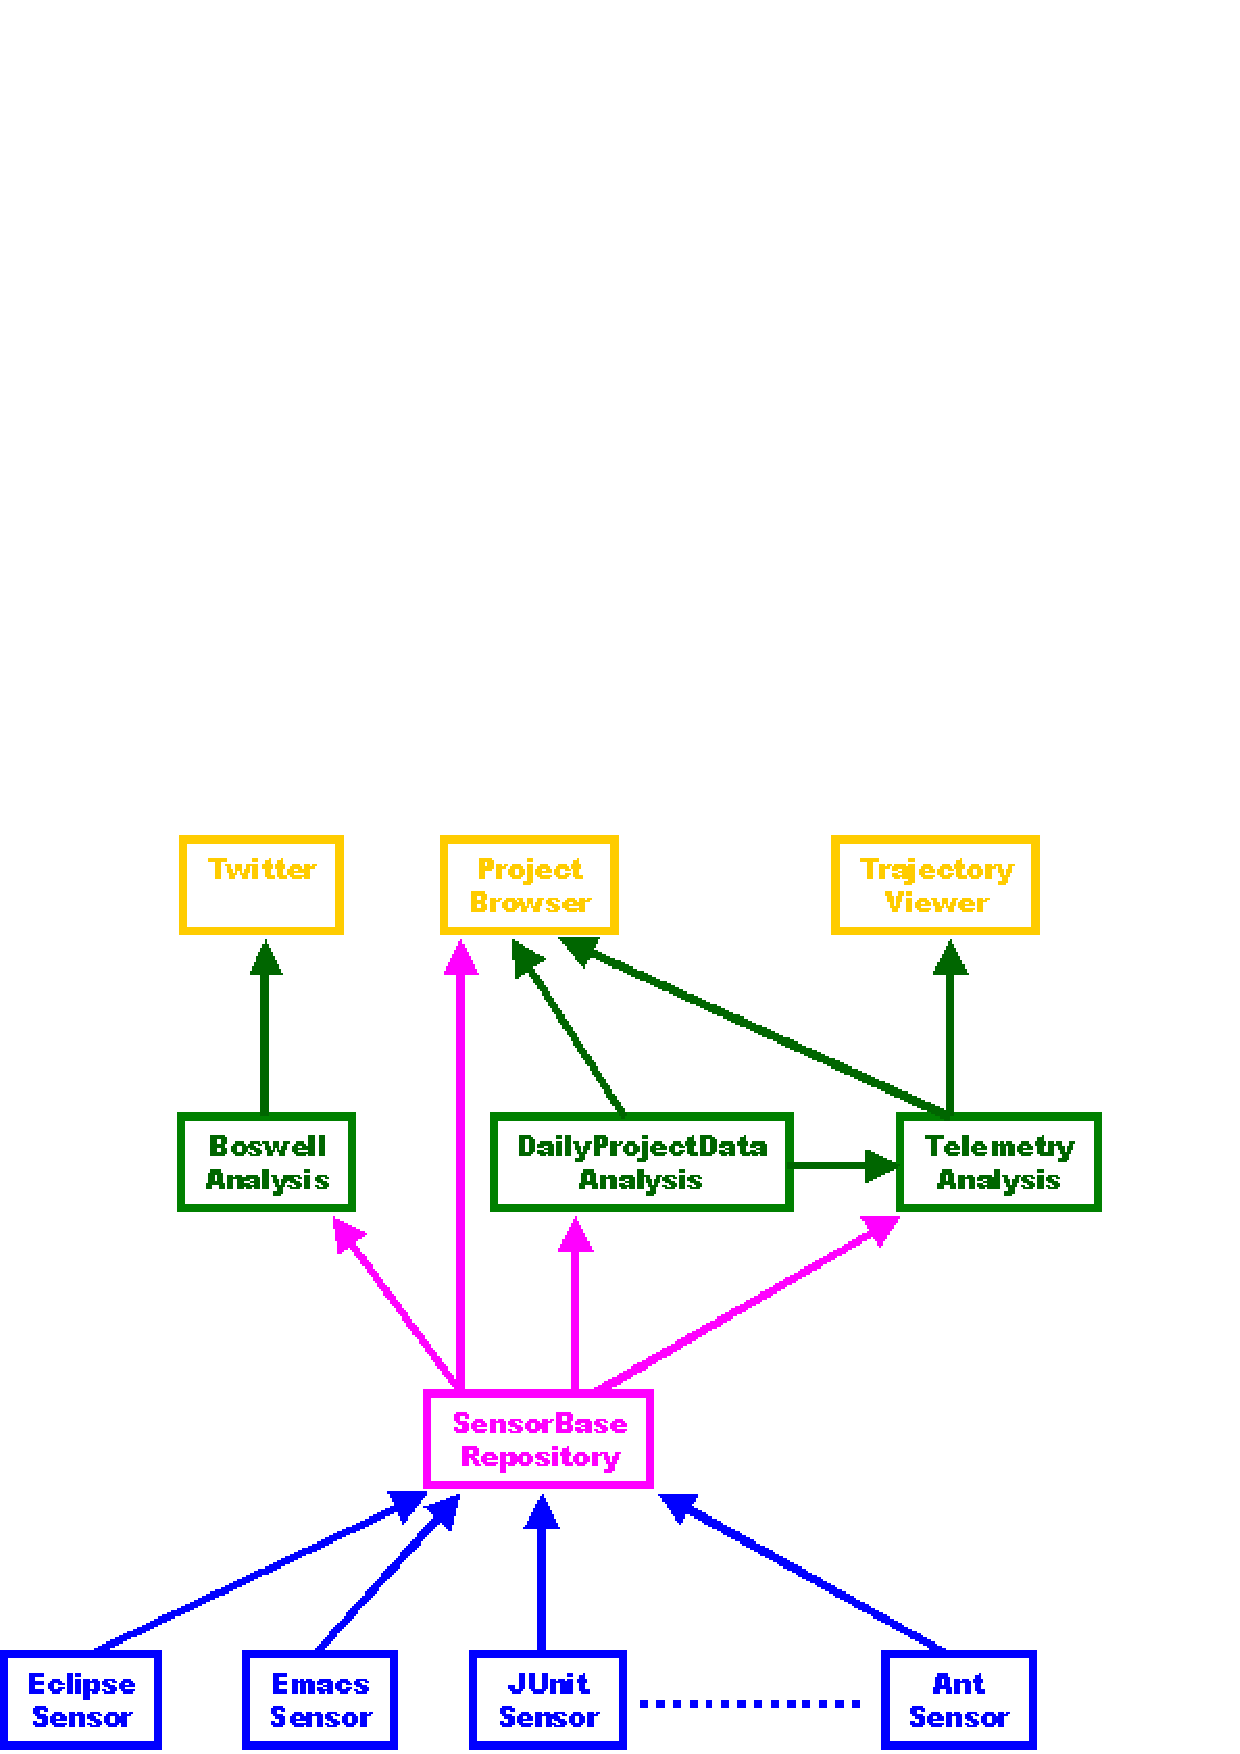
\includegraphics[height=20em]{hackystat-architecture} 
   \caption{Screenshot of file-metric telemetry analysis of Hackystat in 2006}
   \label{fig:hackystat-architecture}
\end{figure}

\subsection{Sensors}
Sensors are small software plugins to collect data from the use of tools and applications. Currently, sensors are available to many development software including Eclipse, Emacs, Ant, etc. Sensor data is represented in XML, and consist of seven basic elements: data owner, resource, timestamp, runtime, tool, Sensor Data Type and properties. The first six are required and the last one is optional. 

Sensor Data Type(SDT) is specified to every piece of sensor data when collected, so that the same type of data can be collected from different tools and higher level services can easily determine which data is relevant to them. Sensor data is designed to record only an piece of atomic data such as size of a single file, thus runtime is use to group data that belongs to the same event, such as the file metric of a project. Properties are additional information for different types of sensor data, such as coverage value for coverage SDT and lines of code for file metric. 

Sensors are designed to work automatically without any attention form user except the initial configuration. In order to reduce internet communication and support offline working, data is temporarily stored in local space, then is sent to data repository every several minutes or when internet connection is available.

\subsection{SensorBase}
Sensor data is sent to the data repository, called SensorBase. SensorBase store the data as it sent from sensors, and provide RESTful interface for easy query. Sensor data can be queried with the six required elements mentioned above via HTTP calls, and data is sent back as XML. SensorBase is implemented with a database manager abstract class, thus it is easy to add support to different database implementations. Current version of Hackystat provides database support for Derby, Oracle and PostgreSQL.

\section{Analysis Services}
Analysis services of Hackystat provide data abstraction of the raw data from SensorBase. DailyProjectData and Telemetry are the two most fundamental analyses of Hackystat.

\subsection{Daily Project Data Analysis}
As its name tells, DailyProjectData(DPD) service provides abstractions of sensor data associated with a single project within a 24 hour period, which represents a simple software development metric in a single day. Data of a single project includes data from all members of that project. In a DailyProjectData instance, both summary value, e.g. total development time across the project, and detail values, e.g. total development time of a project member, are available. So it is easy for higher level service to use this data.

Each DPD analysis generates software metric from data of a certain Sensor Data Type. Current available DPD analyses are Build, Code Issue, Commit, Complexity, Coupling, Coverage, Dev Time, File Metric, Issue, and Unit Test. These DPD analyses are the basic of the Hackystat system, all other analysis services are based on DPD. While DPD is the lowest level of abstraction, these can also be considered as the available software metrics in Hackystat.

\subsection{Telemetry Analysis}
Based on DPD service, Telemetry service provides abstraction over a longer period of time such as several days, weeks or months. A Telemetry Chart consists of one or more streams of data points. Each data point represents the metric value of in a single granularity (day, week or month). Together they show the trend of the metric(s).

There is a special group of Telemetry charts called Member-Level Telemetry. These charts consist of several stream, each of which belongs to a project member. They are used in Software ICU's drill down feature to compare performance of each member within a project. 

To support the work practices of different organizations, Telemetry service provides a domain specific language that allows to build new Telemetry Chart with Telemetry stream lines. The predefined Telemetry Charts are all written with this language.

Telemetry streams can also accept parameters to refine the object data. This feature is inherited in Software ICU, where user can configure the parameters of each Telemetry analysis of each vital sign (more detail discuss in \autoref{vitalSign} and \autoref{SICUconfiguration}).

\section {Project Browser}
Project Browser is one of the viewers in Hackystat system. It is based on Wicket\footnote{\url{http://wicket.apache.org/}}, a Java-based web application framework. Project Browser is integrated with viewers to all Hackystat services, which are organized as tabs. 

With help of Wicket's modularization, viewers on Project Browser can share many common panel, such as project/date selection panel and Ajax loading process panel, which facilitate the development of new page. This also makes user's experience more consistent across different viewers. Therefore it now serves as a data presentation and high level analysis development center. Several new presentations and high level analysis are developed upon it, Software ICU is one them.

\chapter{Design and Implementation of Software ICU}
In order to achieve good management of software development projects, we develop a system called Software Intensive Care Unit consists of a number of software development metrics and use these metrics to generate a number of vital signs that state represent "health" state of software development projects.

\section{Vital Signs}
\label{vitalSign}

Vital signs of software projects are measured by various software development process or product metrics. Each of these metric reveal an aspect of the state of the software project.
\begin{description}
\item[Coverage] 
Coverage is a measure used in software testing. It describes the degree to which the source code of a program has been tested. It measures the quality of the tests, which is an essential part of program quality insurance.
\item[Cyclomatic complexity] 
Cyclomatic complexity, was developed by Thomas J. McCabe and is used to measure the complexity of a program. It directly measures the number of linearly independent paths through a program's source code.\cite{mccabe:complexity} Higher cyclomatic complexity means more distinct control paths in a program module, thus it is more difficult to fully test them and the untested paths may have deficiency inside. Therefore, program modules are preferred to have lower complexity.
\item[Coupling] 
Coupling, or dependency, is the degree to which each program module relies on each one of the other modules.\cite{wiki:coupling} It is actually a measure of the complexity of the whole system's module reference tree. Whenever one module is modified, there will be a chance that the changes may cause bugs in one of modules that relies on this one. Therefore, higher coupling value implies higher risk of introducing bugs when making changes, thus more difficult to maintain the system.
\item[Churn] 
Churn is a measure of the total number of lines of code deleted and added. It represent the amount of changes made to the system, which reflects the work to the system. Interpretation of this metric is conditional. Low churn means low work load to the system, but also means consistency of the system, thus is good for systems under maintenance. However, high churn implies higher inconsistency of the source code of the system, but also means high work load, which is the normal case of a intensively developing project.
\item[Size] 
The size of software program is measured by the source lines of code (SLOC), which counts the number of lines in the text of the program's source code. SLOC is typically used to predict the amount of effort that will be required to develop a program, as well as to estimate programming productivity or effort once the software is produced.
\item[Commit] 
Commit measure the number of commitments made to the source code repository. It is recommended that programmer should make commit often and make it small and keep the integration consistent.
\item[DevTime] 
DevTime, abbreviation of Develop Time, is a measure of total human work put into the system.
\item[Build] 
Build is a count of ant build task invoked in a period of time.
\item[Test] 
Test is a count of unit tests invoked in a period of time.
\end{description}

\section{Vital Sign Presentation}
\subsection{Vital Sign from latest value}
Latest values of software metrics are important enough to be shown separately because they represent the latest state of a project. We assign colors to latest value of the measures to indicate their performing.

\subsection{Vital Sign from historical trend via spark-line}
Historical data of software metric is as good as the latest one. It provides more information of the performance of the project over time. But in the same time it bring a great amount of data overwhelming as well. In order to reduce the historical data to an acceptable small but meaningful degree, we use spark-line to represent them. Then we assign colors to the spark-lines with several evaluation strategies: Stream Trend and Participation.

\subsubsection{Stream Trend Evaluation}
Stream trend evaluation determines the health of a stream by its trend. It takes one parameter called HigherBetter. If user define the higher value the better, then increasing trends will be considered as a healthy trend and decreasing trends will be considered as unhealthy. Stable trends are always considered as healthy because in that case it is as good as health that one don't need to pay too much attention to it, while the actual value will be shown in the latest value where the value will be judged to be good or not. And unstable trend is marked as average because it is not easy to tell if it indicates a good state or not. 

\subsubsection{Participation Evaluation}
Participation evaluation determines the health of a stream by the participations of all members in the project. When working as a group, it is not good that some of the member do most of the work and others do little, thus in this situation the stream will be classified as unhealthy stream, which mean to attract attention.

\section{Mini Chart Drill Down}

\section{Vital Sign Configuration}
\label{SICUconfiguration}

\section{System Customization}

\chapter{Classroom Evaluation}

\chapter{Contribution and Future Directions}

\section{Current Defects}

\subsection{Data Completeness}

DevTime does not show completely the time developers spent on the project. 

Defects: Fail of unit testing and coverage does not necessary indicate the number of defects in the code. Code review data is needed. 


